\documentclass[runningheads,a4paper]{llncs}

\usepackage{amssymb}
\setcounter{tocdepth}{3}
\usepackage{graphicx}
\usepackage{hyperref}
\usepackage{fixltx2e}

\usepackage{url}
\urldef{\mailsa}\path|{i.c.t.m.speek, a.c.stolwijk}@student.tudelft.nl|
\newcommand{\keywords}[1]{\par\addvspace\baselineskip%
\noindent\keywordname\enspace\ignorespaces#1}

\begin{document}

\mainmatter% start of an individual contribution

% first the title is needed
\title{Presentation Plan\\
FF-Replan: \& RFF\@: Exploiting classical AI planning for uncertain and probabilistic domains}

% a short form should be given in case it is too long for the running head
\titlerunning{Presentation Plan}

\author{I.C.T.M Speek, A.C. Stolwijk}

%
\authorrunning{Presentation Plan Seminar Algorithms FF-replan \& RFF}
% (feature abused for this document to repeat the title also on left hand pages)

% the affiliations are given next; don't give your e-mail address
% unless you accept that it will be published
\institute{Seminar Algorithms, Embedded Software,
Msc Embedded Systems,\\
Delft University of Technology\\
\mailsa\\
}

%\toctitle{Lecture Notes in Computer Science}
%\tocauthor{Authors' Instructions}

\maketitle

\section{Introduction to a planner (A)}



Examples of planning problems:

\begin{itemize}
	\item Blocks World
	\item Motion Planning
\end{itemize}

Planning Problem:

\begin{itemize}
	\item Initial State
	\item Goal State
	\item Set of actions
\end{itemize}

Planning Plan:

\begin{itemize}
	\item Set of actions
	\item Executable in the initial state
	\item Resulting in a state that satisfies the goal state
\end{itemize}

\section{What is uncertainty (I)}

\emph{Uncertainty applies to predictions of future events, to physical measurements that are already made, or to the unknown. Uncertainty arises in partially observable and/or stochastic environments, as well as due to ignorance and/or indolence} [1]. \\

Uncertain (adjective). \\
1. not able to be relied on; not known or definite. [2]

In the rest of this topic discuss the different domains and applications.

\subsection{Real world examples}

Growing plants is an extremely uncertain domain. When everything goes well, it should be fine to water it once a week. However my room environment has proven to be an uncertain domain where wind, temperature and sunlight severely impacts my abality to plan for nurturing my plants.

\subsection{Embedded Systems in uncertain domains}

Cruise control (stabilizing systems), quad rotor, AI, robots

\subsection{Benchmarking for uncertain domains}

Traffic control benchmark for the 2014 IPCC probabilistic continuous domain.
Tidybot: a housecleaning robot [3]. \\

\noindent [1] [Wikipedia http://en.wikipedia.org/wiki/Uncertainty]
[2] [Google definition]
[3] [http://www.plg.inf.uc3m.es/ipc2011-deterministic/DomainsSequential.html\#Barman]

\section{Historic Overview}
A swift introduction to the evolution of planning algorithms. For every problem state the:
\begin{itemize}
	\item The problem definition
	\item The motivation for the solution
	\item The strengths
	\item The weaknesses
\end{itemize}

\subsection{$<$ 1990 (A)}

\begin{itemize}
	\item STRIPS \cite{fikes1971strips}
\end{itemize}

\subsubsection{STRIPS}

STRIPS~\cite{fikes1971strips} is a influential method of defining planning
problems.

Take for example~\ref{fig:strips}. R is the robot, B and C are two objects at
places a, b and c. The goal is to achieve the configuration such that B is at
place k and in which C is not at place c. The robot can move to an object and
it can push objects to another position.

\begin{figure}[htb]%
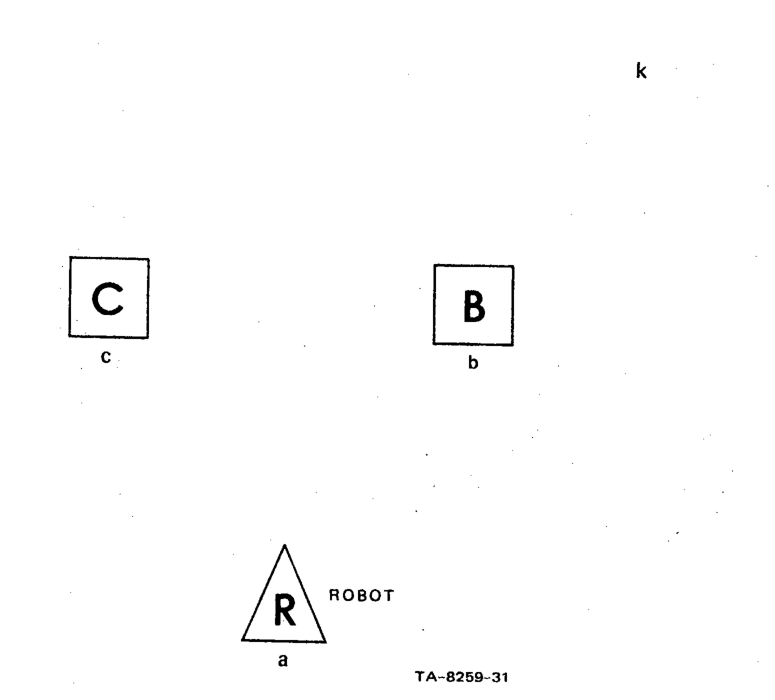
\includegraphics[width=0.8\columnwidth]{strips-example.pdf}%
\caption{Configuration of objects and robot for example problem (Figure from~\cite{fikes1971strips})}%
\label{fig:strips}%
\end{figure}

The goal could be written as

\[
	(\exists s) [ AT(B,k,s) \land \neg AT(C,c,s) ]
\]

If we find an instance of s, the problem is solved.

STRIPS also defines operators. In this instance examples can be \texttt{goto}
and \texttt{push}.

\begin{description}
	\item[push(u,x,y)] Robot pushes object \texttt{u} from \texttt{x} to
		position \texttt{y}
	\begin{description}
		\item[Precondition:] $(\exists s) [AT(u,x,s) \land ATR(x,s)]$
		\item[Delete list:] $\{AT(u,x,s), ATR(x,s)\}$
		\item[Add list:] $\{AT(u,y,push'(u,x,y,s^*)), ATR(y,push'(u,x,y,s^*))\}$
	\end{description}
	\item[goto(x,y)] Robot goes from place \texttt{x} to \texttt{y}
	\begin{description}
		\item[Precondition:] $(\exists s) [ATR(x,s)]$
		\item[Delete list:] $\{ATR(x,s)\}$
		\item[Add list:] $\{ATR(y,goto'(x,y,s^*))\}$
	\end{description}
\end{description}

The initial world model can be described by:

\[
	s_0 : \{ ATR(a,x_0), AT(B,b,s_0), AT(C,c,s_0) \}
\]

Besides that there is a global requirement that two blocks cannot be at the
same position at any time.

\paragraph{Problems}

\begin{itemize}
	\item How to efficiently store nodes (states) of the world.~\cite{fikes1971strips}.
	\item ...
\end{itemize}

\subsection{1990 - 2000 (I)}
Choose 3 of these depending on what comes out in the different era's:

Model Checking, search techniques, least commitment - probabilistic planner (BURIDAN), DMCPs, dynamic programming, graphplan

Still need to check papers, but already have a bunch.


\subsection{Introducing the FF planner (I)}

\subsection{2000 - 2005 (A)}

\subsection{FF-Replan (I)}

\subsection{RFF (A)}

\section{Compare FF-Replan with RFF (I\&A)}

\subsection{How did FF-Replan inspire (I)}

\section{What after? Any new methods (A)}

\section{Present goal of paper (I\&A)}

\section{Is it time to reconsider classical planners (I\&A)}

\bibliographystyle{plain}
\bibliography{Plan_presentation_monday}

\end{document}
